\subsubsection{\nextread}

Once the {\returnpath} gadget has assembled, the counter has a few options to choose from.
%
The gadget that controls what happens after a digit is written is the {\nextread} gadget.
%
If there is a {\tt msr} and {\tt msd} signal in the input, this gadget knows that the most significant digit was just read and will output a
glue for the {\tt Cross\_Next\_Row} gadget to assemble so that the counter crosses
back to the right and begins reading the first digit in the next row.
%
Otherwise (for regular digits not in the MSR), this gadget will assemble the second half of
the return path, terminating at the next digit in the current row.
%
When this happens, the gadget increments the digit index (unless it is already digit 3, in which case it
resets to 1) and outputs an empty {\cread} signal to force the counter to begin reading
the next digit.



For each $\inc\in \{ {\tt increment}, {\tt copy} \}$:
\begin{itemize}

    % DIGIT 1
    \item Create
    $\begin{aligned}[t]
        \nextread(& \left\langle {\tt NextRead},    1,          \inc \right\rangle,
                    \left\langle {\tt CounterRead}, 2, \lambda, \inc \right\rangle \;)
    \end{aligned}$\\from the gadget shown in Figure~\ref{fig:next_read_1-or-2_op}.
    %
    In this step, $2 \cdot \left( 41 + 4l \right) =$
    %
    $82 + 8l =$
    %
    $82 + 8 \cdot \left( \ceil*{\log m} + 2 \right) \leq$
    %
    $82 + 8 \cdot \left( {\log m} + 3 \right) =$
    %
    $106 + 8 \cdot {\log m} = \bigologm$ tiles were created.
    %
    \vspace{0.5cm}

    \item Create
    $\begin{aligned}[t]
        \nextread(& \left\langle {\tt NextRead},    1,          \inc, {\tt msr} \right\rangle,
                    \left\langle {\tt CounterRead}, 2, \lambda, \inc            \right\rangle \;)
    \end{aligned}$\\from the gadget shown in Figure~\ref{fig:next_read_1_op_msr}.
    %
    In this step, $2 \cdot \left( 36 + 4l \right) =$
    %
    $72 + 8l =$
    %
    $72 + 8 \cdot \left( \ceil*{\log m} + 2 \right) \leq$
    %
    $72 + 8 \cdot \left( {\log m} + 3 \right) =$
    %
    $96 + 8 \cdot {\log m} = \bigologm$ tiles were created.
    %
    \vspace{0.5cm}

    \item Create
    $\begin{aligned}[t]
        \nextread(& \left\langle {\tt NextRead}, 1,  \inc, {\tt msr}, {\tt msd} \right\rangle,
                    \left\langle {\tt CrossNextRow}, \inc                       \right\rangle \;)
    \end{aligned}$\\from the gadget shown in Figure~\ref{fig:next_read_1-or-2_op_msr_msd}.
    %
    In this step, $2 \cdot \left( 37 + 4l \right) =$
    %
    $74 + 8l =$
    %
    $74 + 8 \cdot \left( \ceil*{\log m} + 2 \right) \leq$
    %
    $74 + 8 \cdot \left( {\log m} + 3 \right) =$
    %
    $98 + 8 \cdot {\log m} = \bigologm$ tiles were created.
    %
    \vspace{0.5cm}

    % DIGIT 2
    \item Create
    $\begin{aligned}[t]
        \nextread(& \left\langle {\tt NextRead},    2,          \inc \right\rangle,
                    \left\langle {\tt CounterRead}, 3, \lambda, \inc \right\rangle \;)
    \end{aligned}$\\from the gadget shown in Figure~\ref{fig:next_read_1-or-2_op}.
    In this step, $2 \cdot \left( 41 + 4l \right) =$
    %
    $82 + 8l =$
    %
    $82 + 8 \cdot \left( \ceil*{\log m} + 2 \right) \leq$
    %
    $82 + 8 \cdot \left( {\log m} + 3 \right) =$
    %
    $106 + 8 \cdot {\log m} = \bigologm$ tiles were created.
    %
    \vspace{0.5cm}

    \item Create
    $\begin{aligned}[t]
        \nextread(& \left\langle {\tt NextRead}, 2,  \inc, {\tt msr}, {\tt msd} \right\rangle,
                    \left\langle {\tt CrossNextRow}, \inc                       \right\rangle \;)
    \end{aligned}$\\from the gadget shown in Figure~\ref{fig:next_read_1-or-2_op_msr_msd}. In this step $37 + 4l$ tiles were created.
    %
    In this step, $2 \cdot \left( 37 + 4l \right) =$
    %
    $74 + 8l =$
    %
    $74 + 8 \cdot \left( \ceil*{\log m} + 2 \right) \leq$
    %
    $74 + 8 \cdot \left( {\log m} + 3 \right) =$
    %
    $98 + 8 \cdot {\log m} = \bigologm$ tiles were created.
    %
    \vspace{0.5cm}

    % DIGIT 3
    \item Create
    $\begin{aligned}[t]
        \nextread(& \left\langle {\tt NextRead},    3,          \inc \right\rangle,
                    \left\langle {\tt CounterRead}, 1, \lambda, \inc \right\rangle \;)
    \end{aligned}$\\from the gadget shown in Figure~\ref{fig:next_read_3_op}. In this step $94 + 12l$ tiles were created.
    %
    In this step, $2 \cdot \left( 94 + 12l \right) =$
    %
    $188 + 24l =$
    %
    $188 + 24 \cdot \left( \ceil*{\log m} + 2 \right) \leq$
    %
    $188 + 24 \cdot \left( {\log m} + 3 \right) =$
    %
    $260 + 24 \cdot {\log m} = \bigologm$ tiles were created.
    %
    \vspace{0.5cm}

    \item Create
    $\begin{aligned}[t]
        \nextread(& \left\langle {\tt NextRead}, 3,  \inc, {\tt msr}, {\tt msd} \right\rangle,
                    \left\langle {\tt CrossNextRow}, \inc \right\rangle \;)
    \end{aligned}$\\from the gadget shown in Figure~\ref{fig:next_read_3_op-or-seed_msr_msd}.
    %
    In this step, $12 = O\left( 1 \right)$ tiles were created.
    %
\end{itemize}

\begin{figure}[H]
    \centering
    \subcaptionbox{
        Digit 1 \& 2 - general. There are $41 + 4l$ tiles in this gadget.
        \label{fig:next_read_1-or-2_op}
    }{\makebox[0.24\textwidth][c]{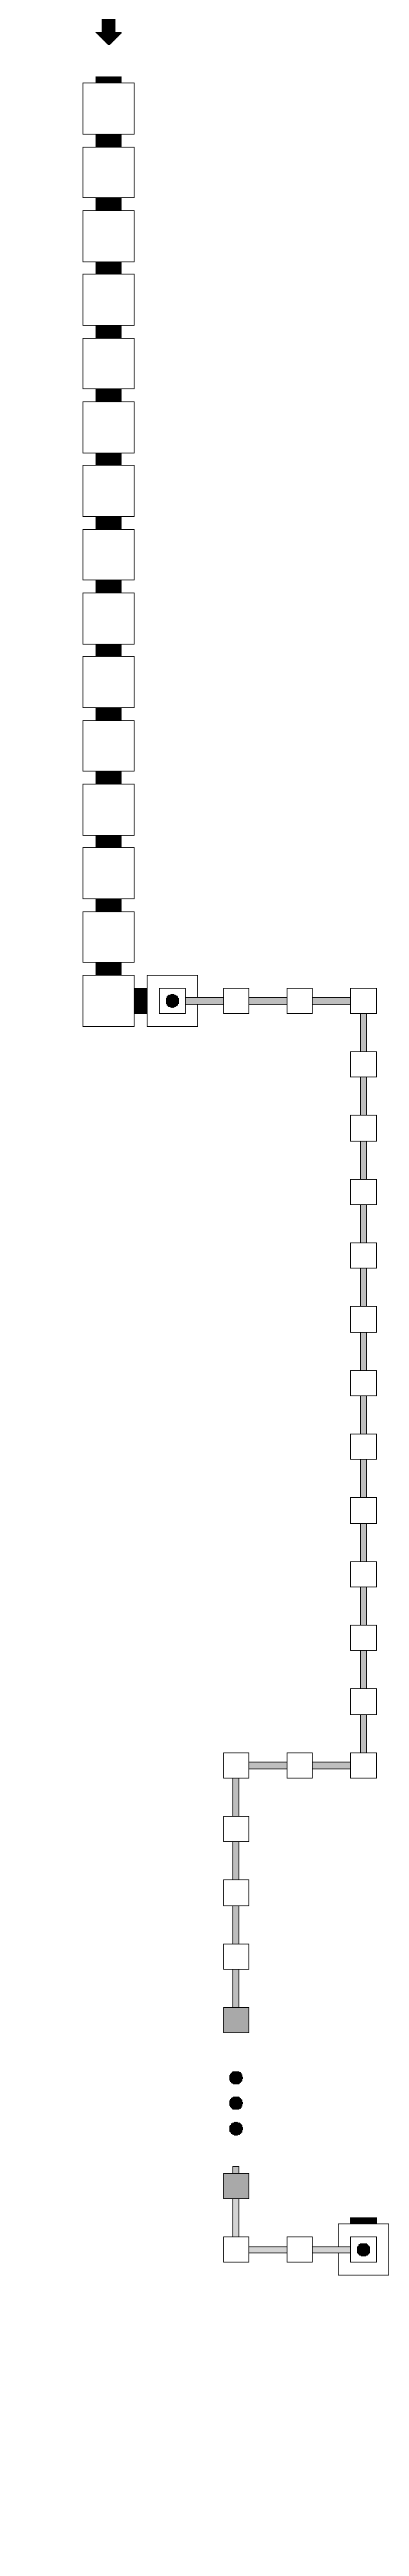
\includegraphics[width=0.45in]{next_read_1-or-2_op}}}%
    ~
    \subcaptionbox{
        Digit 1 - general\\overview.
        The black tiles in this figure correspond to the gadget shown in subfigure~\subref{fig:next_read_1-or-2_op}.
        \label{fig:next_read_1_op_overview}
    }{\makebox[0.24\textwidth][c]{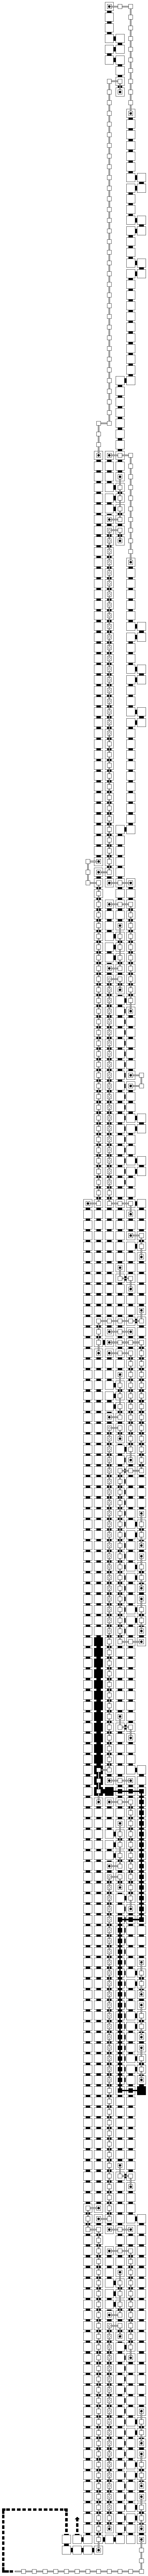
\includegraphics[width=0.45in]{overviews/general/next_read_1_op}}}%
    ~
    \subcaptionbox{
        Digit 1 - general (seed) overview.
        The black tile in this figure is a single tile gadget used only in the initial value.
        \label{fig:next_read_1_seed_op_overview}
    }{\makebox[0.24\textwidth][c]{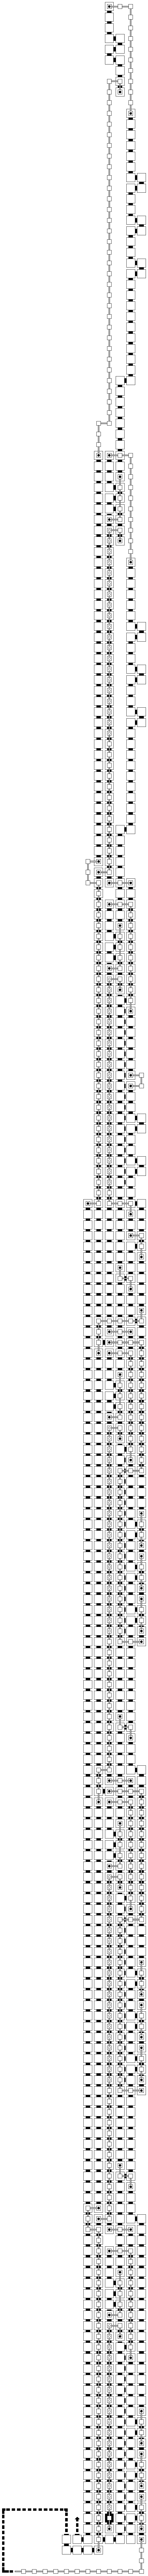
\includegraphics[width=0.45in]{overviews/general/next_read_1_seed_op}}}%
    ~
    \subcaptionbox{
        Digit 2 - general\\overview.
        The black tiles in this figure correspond to the gadget shown in subfigure~\subref{fig:next_read_1-or-2_op}.
        \label{fig:next_read_2_op_overview}
    }{\makebox[0.24\textwidth][c]{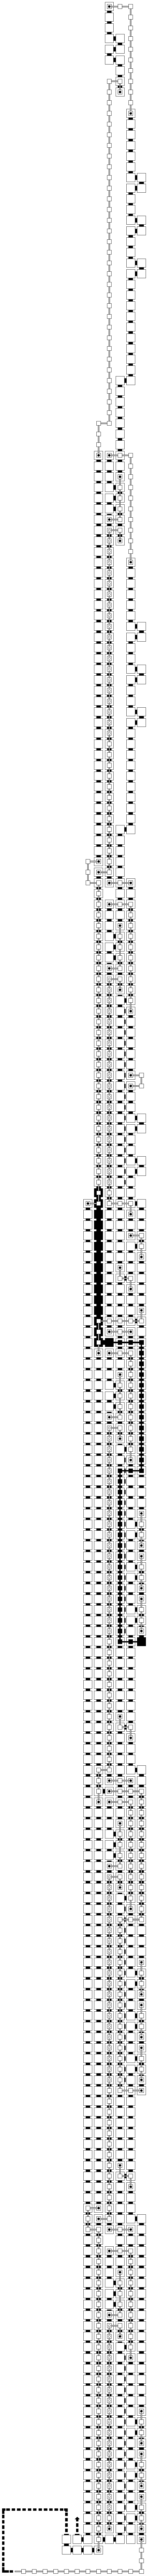
\includegraphics[width=0.45in]{overviews/general/next_read_2_op}}}%
    ~
\end{figure}
\begin{figure}[H]\ContinuedFloat
    \centering
    \subcaptionbox{
        Digit 3 - general. There are $94 + 12l$ tiles in this gadget.
        \label{fig:next_read_3_op}
    }{\makebox[0.24\textwidth][c]{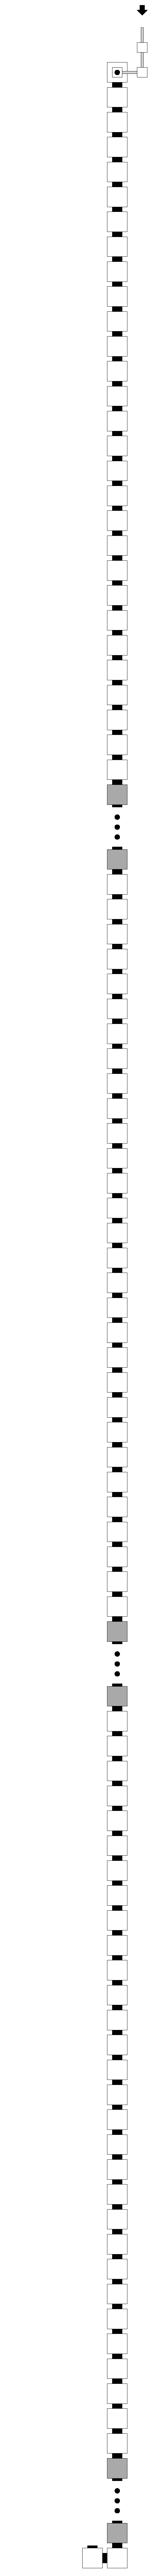
\includegraphics[width=0.45in]{next_read_3_op}}}%
    ~
    \subcaptionbox{
        Digit 3 - general\\ overview.
        The black tiles in this figure correspond to the gadget shown in subfigure~\subref{fig:next_read_3_op}.
        \label{fig:next_read_3_op_overview}
    }{\makebox[0.24\textwidth][c]{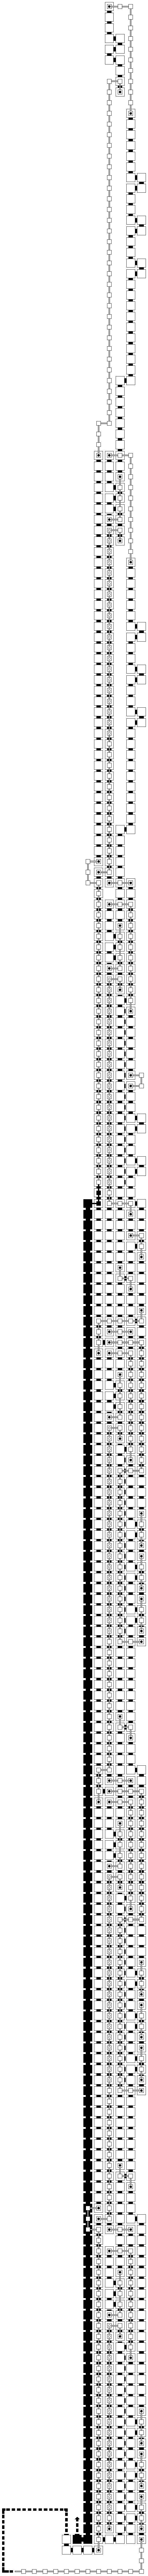
\includegraphics[width=0.45in]{overviews/general/next_read_3_op}}}%
    ~
    \subcaptionbox{
        Digit 2 - seed. There are $3$ tiles in this gadget.
        \label{fig:next_read_2_seed_op}
    }{\makebox[0.24\textwidth][c]{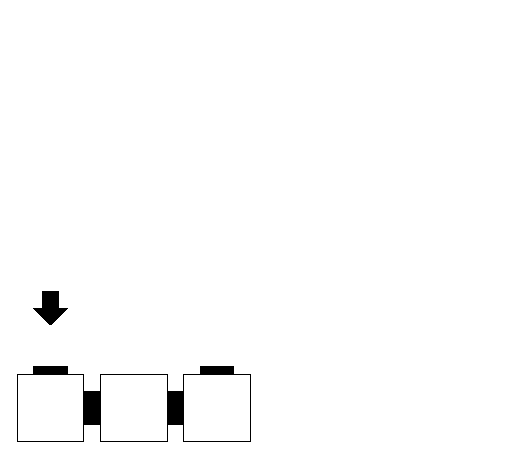
\includegraphics[width=0.45in]{next_read_2_seed}}}%
    ~
    \subcaptionbox{
        Digit 2 - seed overview.
        The black tiles in this figure correspond to the gadget shown in subfigure~\subref{fig:next_read_2_seed_op}.
        \label{fig:next_read_2_seed_op_overview}
    }{\makebox[0.24\textwidth][c]{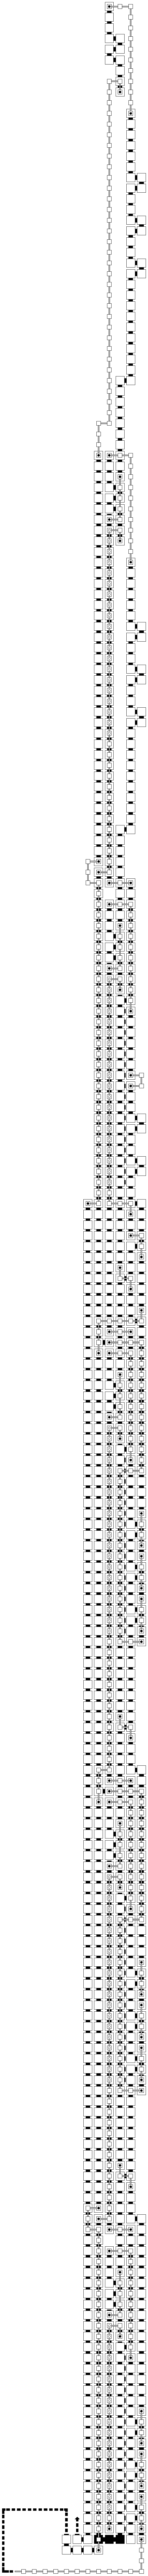
\includegraphics[width=0.45in]{overviews/general/next_read_2_seed_op}}}%
    ~
\end{figure}
\begin{figure}[H]\ContinuedFloat
    \centering
    \subcaptionbox{
        Digit 3 - seed. There are $7$ tiles in this gadget.
        \label{fig:next_read_3_seed_op}
    }{\makebox[0.24\textwidth][c]{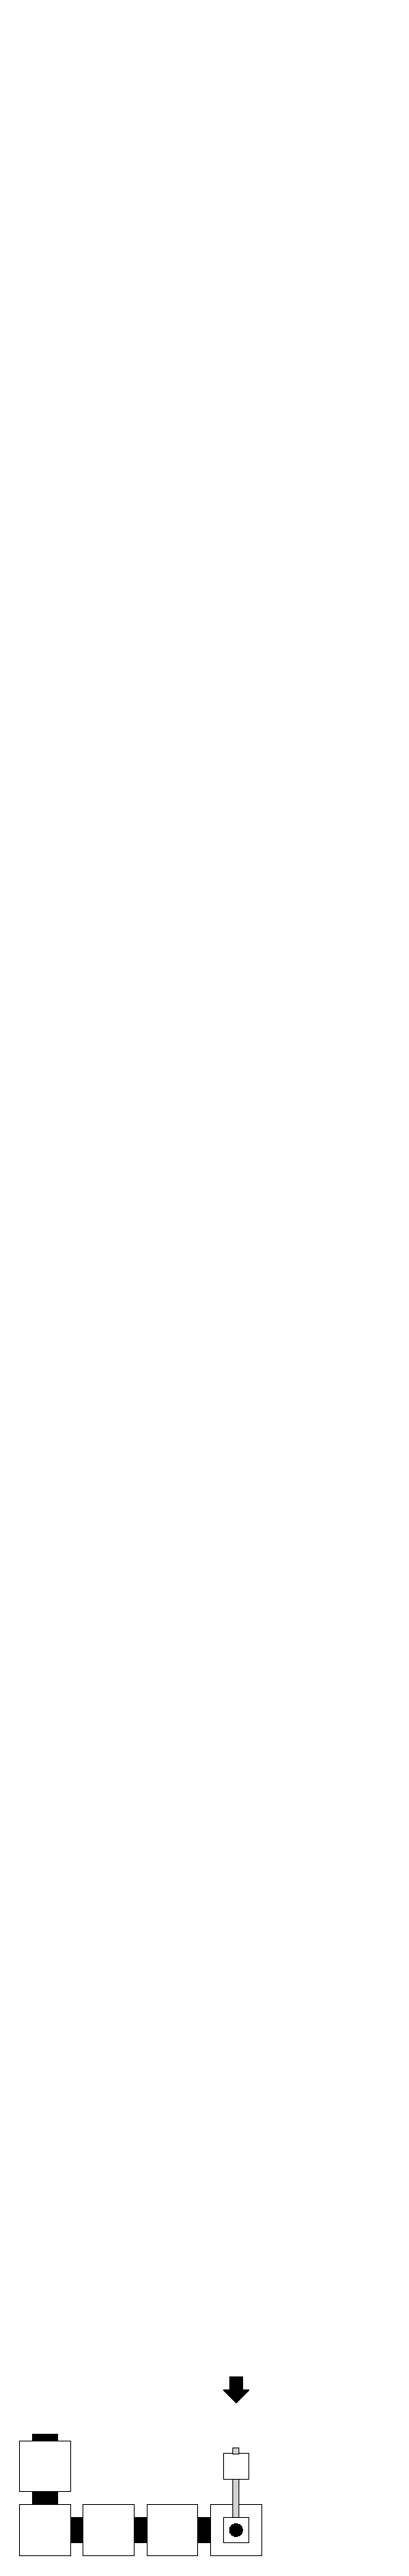
\includegraphics[width=0.45in]{next_read_3_seed}}}%
    ~
    \subcaptionbox{
        Digit 3 - general (seed) overview.
        The black tiles in this figure correspond to the gadget shown in subfigure~\subref{fig:next_read_3_seed_op}.
        \label{fig:next_read_3_seed_op_overview}
    }{\makebox[0.24\textwidth][c]{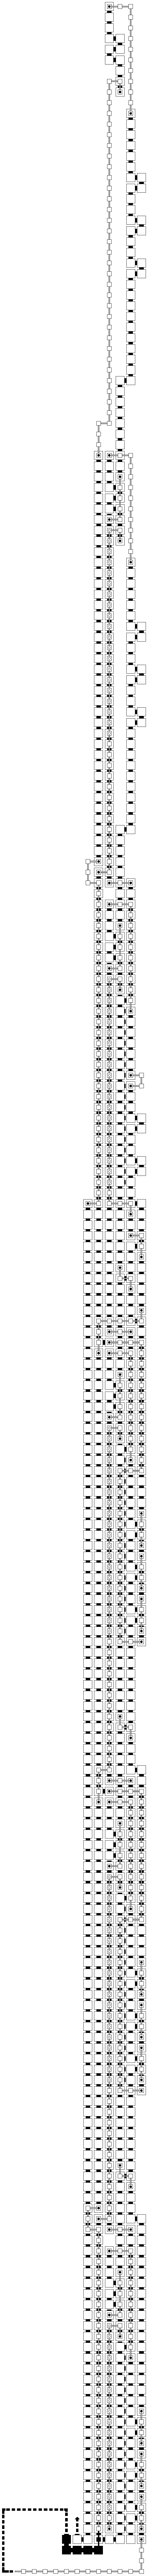
\includegraphics[width=0.45in]{overviews/general/next_read_3_seed_op}}}%
    ~
    \subcaptionbox{
        Digit 1 - case 1,\\Digit 2 - case 2. There are $37 + 4l$ tiles in this gadget.
        \label{fig:next_read_1-or-2_op_msr_msd}
    }{\makebox[0.24\textwidth][c]{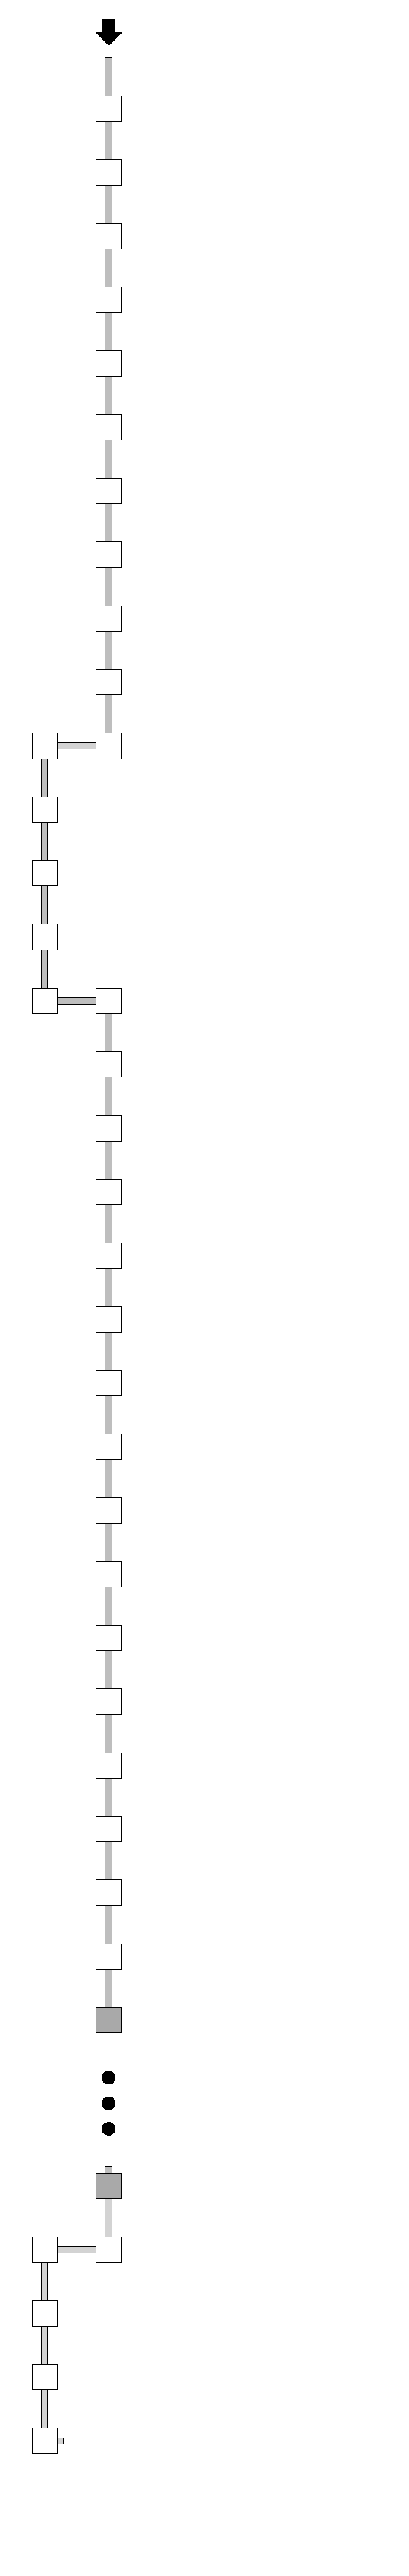
\includegraphics[width=0.45in]{next_read_1-or-2_op_msr_msd}}}%
    ~
    \subcaptionbox{
        Digit 1 - case 1 overview.
        The black tiles in this figure correspond to the gadget shown in subfigure~\subref{fig:next_read_1-or-2_op_msr_msd}.
        \label{fig:next_read_1_op_msr_msd_overview}
    }{\makebox[0.24\textwidth][c]{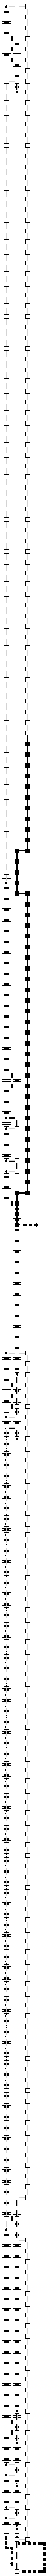
\includegraphics[width=0.45in]{overviews/case1/next_read_1_op_msr_msd}}}%
    ~
\end{figure}
\begin{figure}[H]\ContinuedFloat
    \centering
    \subcaptionbox{
        Digit 2 - case 2\\overview.
        The black tiles in this figure correspond to the gadget shown in subfigure~\subref{fig:next_read_1-or-2_op_msr_msd}.
        \label{fig:next_read_2_op_msr_msd_overview}
    }{\makebox[0.24\textwidth][c]{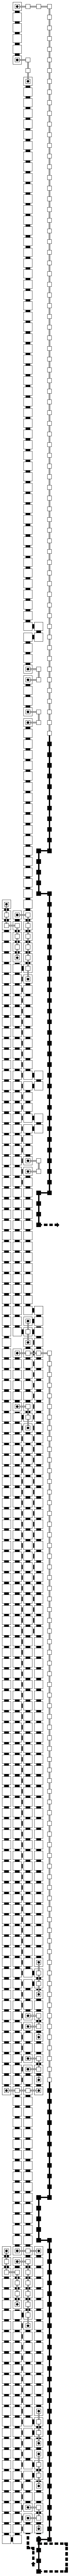
\includegraphics[width=0.45in]{overviews/case2/next_read_2_op_msr_msd}}}%
    ~
    \subcaptionbox{
        Digit 2 - case 2 (seed) overview.
        The black tiles in this figure correspond to the gadget shown in subfigure~\subref{fig:next_read_1-or-2_op_msr_msd}.
        \label{fig:next_read_2_seed_op_msr_msd_overview}
    }{\makebox[0.24\textwidth][c]{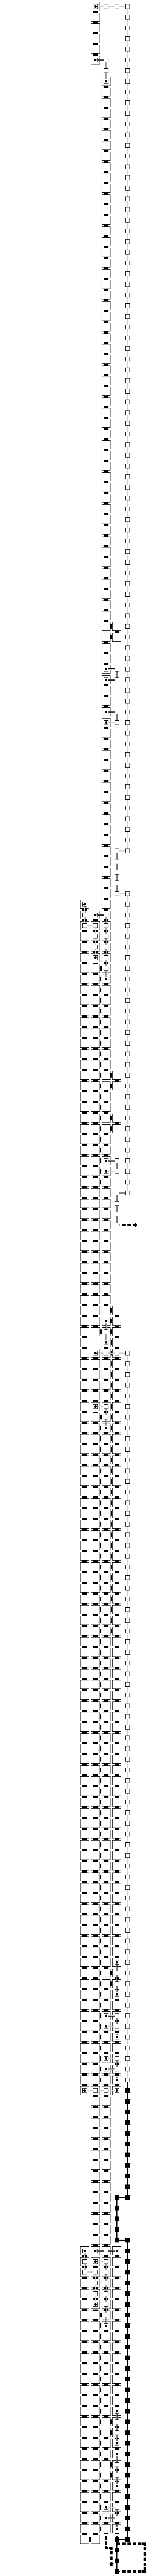
\includegraphics[width=0.45in]{overviews/case2/next_read_2_seed_op_msr_msd}}}%
    ~
    \subcaptionbox{
        Digit 1 - case 2. There are $36 + 4l$ tiles in this gadget.
        \label{fig:next_read_1_op_msr}
    }{\makebox[0.24\textwidth][c]{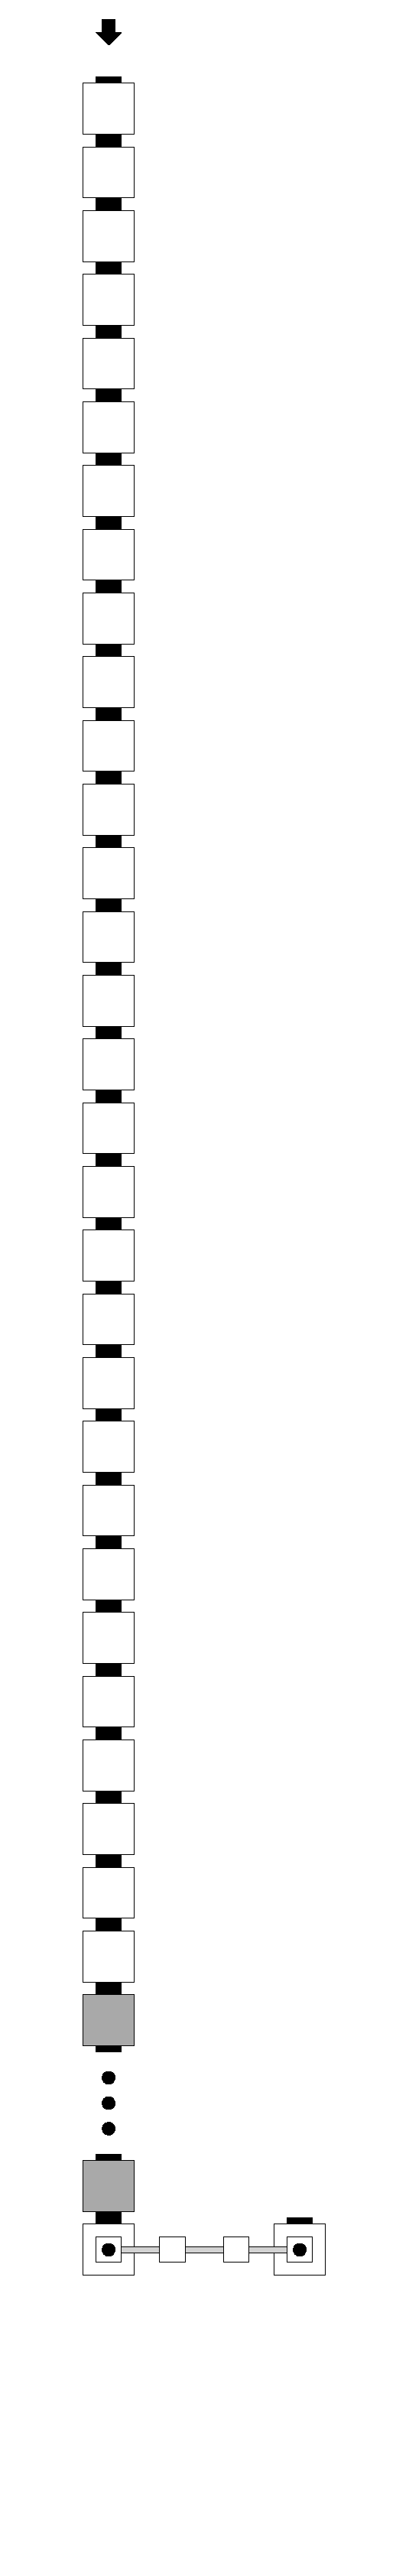
\includegraphics[width=0.45in]{next_read_1_op_msr}}}%
    ~
    \subcaptionbox{
        Digit 1 - case 2 overview.
        The black tiles in this figure correspond to the gadget shown in subfigure~\subref{fig:next_read_1_op_msr}.
        \label{fig:next_read_1_op_msr_overview}
    }{\makebox[0.24\textwidth][c]{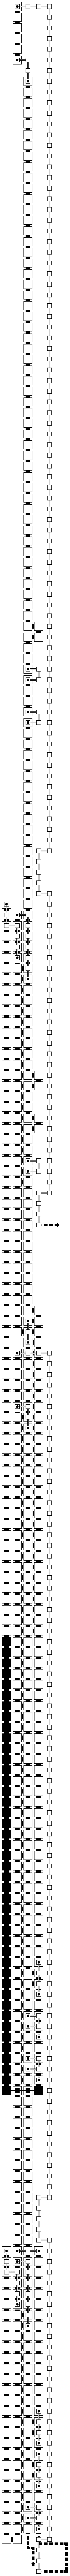
\includegraphics[width=0.45in]{overviews/case2/next_read_1_op_msr}}}%
    ~
\end{figure}
\begin{figure}[H]\ContinuedFloat
    \centering
    \subcaptionbox{
        Digit 3 - case 3. There are $12$ tiles in this gadget.
        \label{fig:next_read_3_op-or-seed_msr_msd}
    }{\makebox[0.24\textwidth][c]{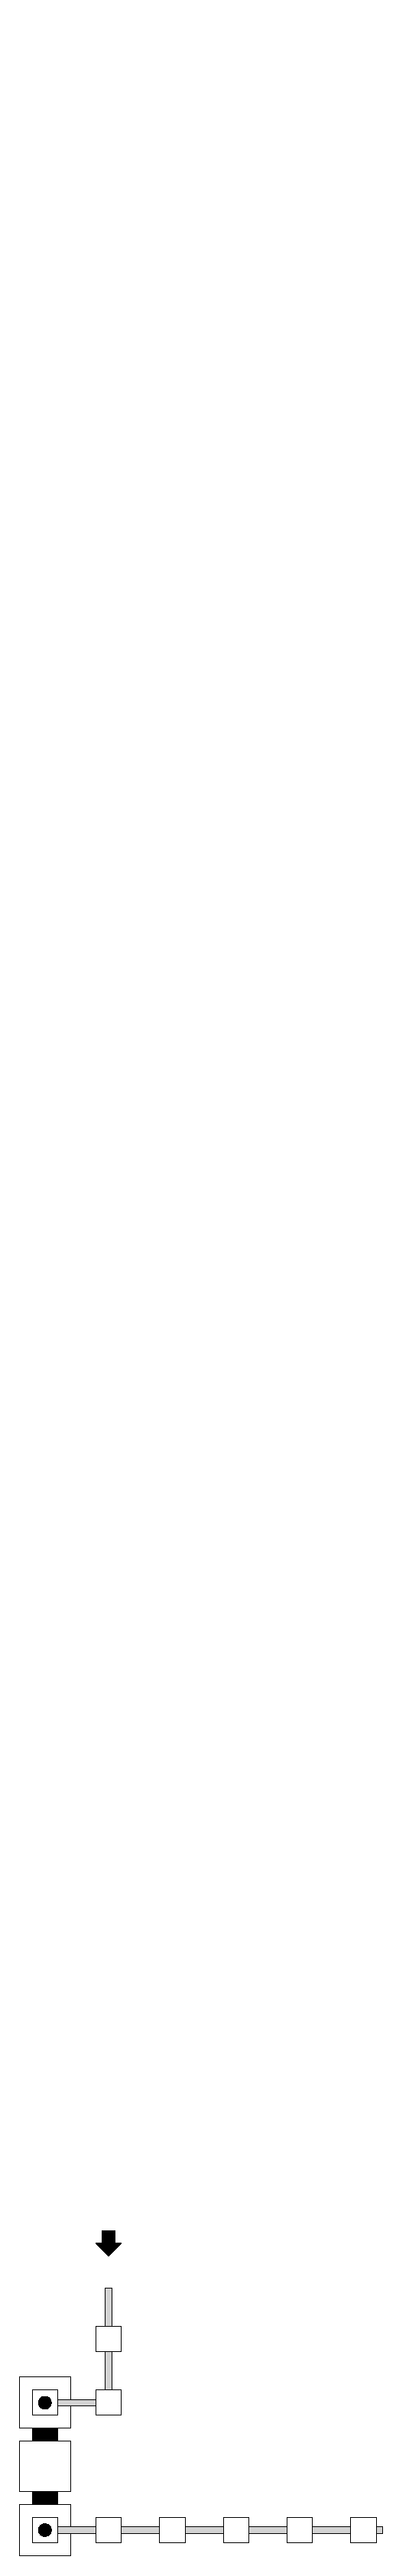
\includegraphics[width=0.45in]{next_read_3_op-or-seed_msr_msd}}}%
    ~
    \subcaptionbox{
        Digit 3 - case 3 overview.
        The black tiles in this figure correspond to the gadget shown in subfigure~\subref{fig:next_read_3_op-or-seed_msr_msd}.
        \label{fig:next_read_3_op_msr_msd_overview}
    }{\makebox[0.24\textwidth][c]{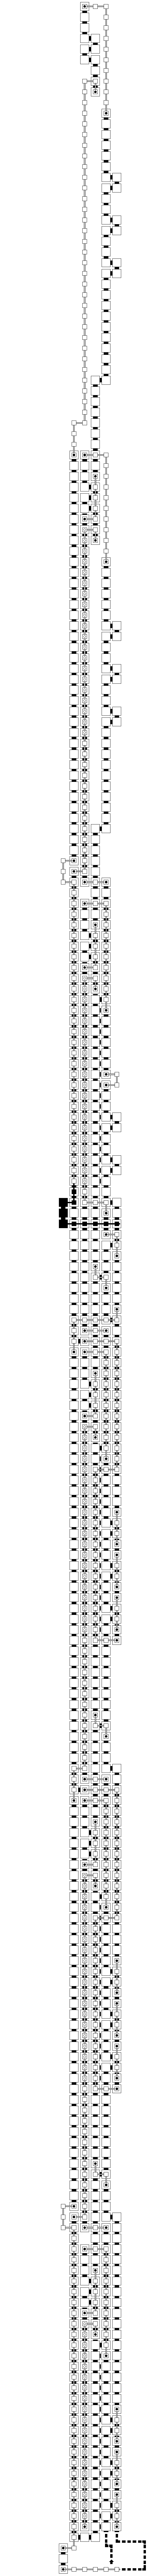
\includegraphics[width=0.45in]{overviews/case3/next_read_3_op_msr_msd}}}%
    ~
    \subcaptionbox{
        Digit 3 - case 3 (seed) overview.
        The black tiles in this figure correspond to the gadget shown in subfigure~\subref{fig:next_read_3_op-or-seed_msr_msd}.
        \label{fig:next_read_3_seed_op_msr_msd_overview}
    }{\makebox[0.24\textwidth][c]{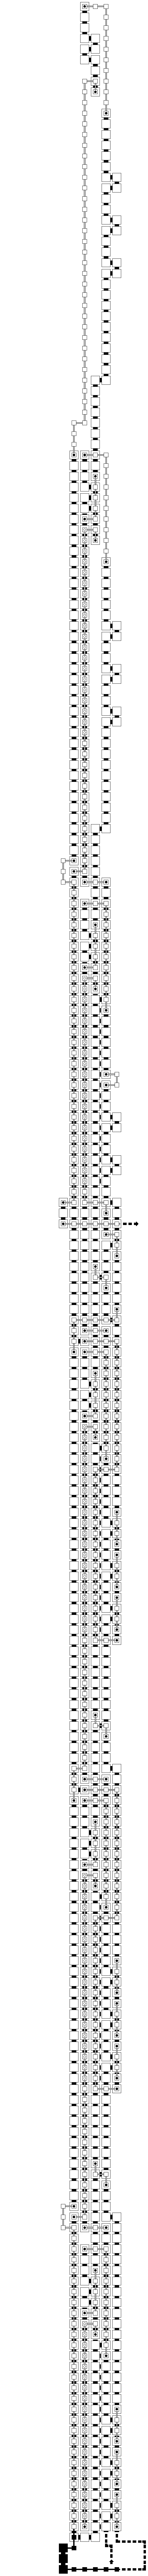
\includegraphics[width=0.45in]{overviews/case3/next_read_3_seed_op_msr_msd}}}%
    ~
    \caption{\label{fig:next_read_gadgets} The {\nextread} gadgets.}
\end{figure}


